\documentclass[uplatex,dvipdfmx,a4paper,10pt]{jsarticle}

\usepackage{amsmath,amsthm,amssymb}
\usepackage[dvipdfmx]{graphicx}
\usepackage{bm}
%
\usepackage{multirow}
\usepackage{wrapfig}

\usepackage{geometry}
\geometry{left=25truemm, right=25truemm, top=25truemm, bottom=25truemm}

%
\abovecaptionskip=-1pt
%\belowcaptionskip=-1pt
%
\renewcommand{\baselinestretch}{0.84} %全体の行間調整
\renewcommand{\figurename}{Fig.}
\renewcommand{\tablename}{Tab.}
%
\makeatletter 
\def\section{\@startsection {section}{1}{\z@}{1.5 ex plus 2ex minus -.2ex}{0.5 ex plus .2ex}{\large\bf}}
\def\subsection{\@startsection{subsection}{2}{\z@}{0.2\Cvs \@plus.5\Cdp \@minus.2\Cdp}{0.1\Cvs \@plus.3\Cdp}{\reset@font\normalsize\bfseries}}
\makeatother 
%

\renewcommand{\thefootnote}{\fnsymbol{footnote}}

\pagestyle{empty}

\graphicspath{{../../figures//}}

\begin{document}

%%%%%%
% はじめに
%%%%%%
\begin{center}
{\Large \textgt{ランダムな接続性を有するネットワークポリマーの緩和挙動}}
\end{center}

\begin{flushright}
東亞合成 ${}^\circ$佐々木裕
\end{flushright}

% \renewcommand{\thefootnote}{\fnsymbol{footnote}}
\footnote[0]{
{\bf Relaxation Characteristics of Network Polymers with random connectivity using Molecular Dynamics Simulations} \\
\underline{Hiroshi SASAKI} (Toagosei Co., Ltd. 8, Showa-Cho, Minato-ku, NAGOYA 455-0026, JAPAN)\\
Tel: +81-52-611-9923, e-mail: hiroshi\_sasaki$@$mail.toagosei.co.jp
}

\vspace{-3mm}
\section{はじめに}

近年、ソフトマターの階層的な構造設計の考え方が深化し、力学特性に優れたネットワークポリマーの材料設計にも応用されている。


ネットワークポリマー研究の深化と新規材料への展開

旧知の材料であるゴムの大きな破壊靭性の由来については、 ヒステリシスロスのようなエネルギー散逸により亀裂進展が抑制されるという Andrews モデルが提案されている\cite{andrews}。
また、ゴム系材料の破壊において粘弾性挙動として時間温度換算則が大変形を伴う破壊挙動にも成立し、室温では容易に破断する SBR がガラス転移温度に近い低温での伸長では高い伸びと強度を示すことも報告されている~\cite{smith}。

ゴム弾性の古典的なモデルである ``Affine Network Model'' からの発展形として、結節点の揺らぎに注目した``Phantom Network Model: PNM''が提案され、Flory によればメルト状態と同一なストランドのゆらぎを有するランダムネットワークにおいて PNM のふるまいを示すとされている~\cite{flory}。
我々は、この結節点のゆらぎ由来の散逸が、分子鎖描像のようなミクロなスケールでの粘弾性的なエネルギー散逸モデルとなりうるのではないかと考え、これまで検討を進めている。
以前に、規則構造ネットワークをベースとしてユニットセル間における規則性をランダムへと変えることで架橋欠損のないネットワークを作成して PNM を再現できることを報告した~\cite{sasaki}。
本報告では、ランダムな接続性を有するネットワークポリマーの緩和挙動について、MD シミュレーションにより検討した結果について報告する。






近年、ソフトマターの階層的な構造設計の考え方が深化し、力学特性に優れたネットワークポリマーの材料設計にも応用されている。
旧知の材料であるゴムの大きな破壊靭性の由来については、 ヒステリシスロスのようなエネルギー散逸により亀裂進展が抑制されるという Andrews モデルが提案されている\cite{andrews}。
また、ゴム系材料の破壊において粘弾性挙動として時間温度換算則が大変形を伴う破壊挙動にも成立し、室温では容易に破断する SBR がガラス転移温度に近い低温での伸長では高い伸びと強度を示すことも報告されている~\cite{smith}。

ゴム弾性の古典的なモデルである ``Affine Network Model'' からの発展形として、結節点の揺らぎに注目した``Phantom Network Model: PNM''が提案され、Flory によればメルト状態と同一なストランドのゆらぎを有するランダムネットワークにおいて PNM のふるまいを示すとされている~\cite{flory}。
我々は、この結節点のゆらぎ由来の散逸が、分子鎖描像のようなミクロなスケールでの粘弾性的なエネルギー散逸モデルとなりうるのではないかと考え、これまで検討を進めている。
以前に、規則構造ネットワークをベースとしてユニットセル間における規則性をランダムへと変えることで架橋欠損のないネットワークを作成して PNM を再現できることを報告した~\cite{sasaki}。
本報告では、ランダムな接続性を有するネットワークポリマーの緩和挙動について、MD シミュレーションにより検討した結果について報告する。



%\subsection{ネットワークポリマー研究の深化と新規材料への展開}
% (ネットワークポリマー研究の深化と新規材料への展開)


% これらの応用として構造材料の軽量化に繋がる新規複合材料の開発が進んでいる。
% その際、一次的な力学的特性の高さだけでなく、長期使用を想定した「破壊」や「疲労」への耐久性が重要となる。
% 高分子材料の耐久性保証を行うためにも、力学特性の発現機構およびその劣化機構の解明が望まれている。

%\subsection{破壊にたいする粘弾性効果}
% (破壊にたいする粘弾性効果)
% 破壊工学の考え方を端的に表せば、「系中に欠損が存在することを前提にした耐久性の評価」ということになろう。
% 脆性破壊する材料を想定した「Griffith 理論」での亀裂進展に伴うエネルギー開放率 $G_c$、さらには、$J$ 積分により非線形領域へ拡張された $J_c$ により破壊挙動が議論され、これらの値が靭性の指標となるとされている。
% しかしながら、破断時の変形がけた違いに大きいソフトマター系の材料への適応には注意が必要である。




%\subsection{力学的ヒステリシスの重要性}
% (力学的ヒステリシスの重要性)
% Andrews は、応力 - ひずみ関係における力学的ヒステリシスに着目し、ヒステリシスロスの存在により亀裂進展に伴うエネルギー開放量が減少し、結果として亀裂の進展が抑制されるモデルを提案している~\cite{Andrews1977}。
% 確かに、上述のゴムにおけるフィラーの効果~\cite{Igarashi2013}、および、DN ゲルにおける犠牲結合~\cite{Gong2010}においては大きなヒステリシスが存在し、その高靭性メカニズムはこの考え方に合致している。

% これらの例はいずれも分子鎖描像より若干大きいメゾスケール領域での挙動であり、この相対的に大きなスケールでの挙動は一般に長時間緩和となる。
% ヒステリシス挙動はこのスケールでしか発現しないのであろうか。
% 我々は、よりミクロな分子鎖描像からも、力学的ヒステリシスによる破壊耐性の向上の可能性があるのではないかと考えている。




%\subsection{疲労に対しての可逆性の重要性}
%
%一般に、破壊試験による材料の強度評価は任意の変形速度での一回の変形挙動で評価されるため、ヒステリシスの回復挙動の遅速はあまり問題にならない。
%しかしながら、材料としての耐久性を保証するためには、多様な変形速度での繰り返し変形を行う疲労試験に対する耐久性も重要である。
%この場合、適正な緩和時間で回復する可逆的なメカニズムに基づく強靭化機構が必要となる。
%
%\subsection{目指すもの}
%



%\subsection{本検討内容}
% (本検討内容)
% ソフトマターの構造材料への展開を標語的に言えば、「脆性破壊を伴いがちな剛直性から、設計された延性に基づく高耐久性を示す『しなやかな強さ』へのパラダイムシフト」となるであろう。
% この設計された延性に必要な要件を明確にすることが本研究の目的である。

% 本報告では、先行研究である Everaers らの方法~\cite{Everaers1999} に従った規則構造を有するネットワークの分子動力学(MD)シミュレーションによりそのゴム弾性挙動の変形速度依存性と緩和時間との関連について検討を行い、時間温度換算則が成り立つような線形粘弾性の枠組みでのヒステリシスを考察した。

\vspace{-1mm}
\section{結果}
\subsection{シミュレーションについて}
既報~\cite{sasaki}に従い、ランダムな接続性を有する 4 および 3 分岐のネットワークを作成し、その平衡状態および変形(一軸伸張およびずりせん断)時の振る舞いについて、OCTA 上の COGNAC シミュレーターを用いた分子動力学シミュレーションにより評価した。


% \subsection{ネットワークの線形粘弾性}
% 変形速度を変化させた場合の SS カーブを Fig.\ref{fig:stretch} に示した。
% 平衡状態の MD シミュレーションから Green-Kubo 公式により求めたネットワークの応力緩和関数(赤線)および $\nu k_B T$ から算出したゴム弾性プラトーの値を緩和関数から差し引いたもの(緑線)を併せて Fig.\ref{fig: Relux} に示した。
% また、ストランドと同等な自由鎖(N=46)のラウス緩和(最長ラウス緩和時間 $\tau_R = 2700$)についても示している。

% この類似性から、少なくとも、今回検討した単純な規則構造を有するネットワークにおいては、架橋構造の緩和時間への寄与は少ないものと推定できた。

% % \begin{wrapfigure}{r}{65mm}
% % %\vspace{-1\baselineskip}
% % 	\begin{center}
% % 	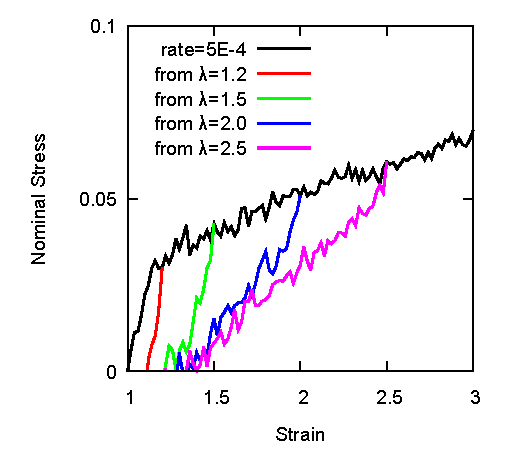
\includegraphics[width=60mm]{./fig/N44_rev_SS.pdf}
% % 	\caption{Hysteresis Curves from different elongation position}
% % 	\label{fig: hyst}
% % 	\end{center}
% % \vspace{-5mm}
% % \end{wrapfigure}

\subsection{力学応答の評価}
4 分岐のネットワークポリマーに対して、変形速度の異なるせん断変形(1e-2 $\sim$ 5e-5 $\lambda/\tau$)時の SS カーブを、各種モデルの理論曲線と共に Fig. \ref{fig:deform} に示した。
変形速度の低減により、$\lambda<1$ 程度の小さなひずみでは PNM に漸近していた。
PNM へと漸近する変形速度 (2e-4 $\lambda/\tau$) で周期的なせん断変形 ($\lambda = 1$) を付与した結果(Fig. \ref{fig:hyst})においても、複数回の変形に対しても迅速な回復を伴った力学的ヒステリシス (Hysteresis loss $\simeq$ 35\%) を示すことが確認できた。
% また、伸長速度を遅くすることにより、ヒステリシス強度が減少することも確認できた。

変形モードの違いによって上記の挙動が変化することも見出しており、その詳細についても報告予定である。

% \section{おわりに}

% 本報告においては、単純な規則構造を有するネットワークの線形緩和現象と任意の変形速度での力学応答との関係から力学的ヒステリシスが生じることを確認し、その発現メカニズムがストランドの緩和現象に起因するものであることを推定した。
% 実際の破壊現象はこれほど単純ではなく、大変形時の非線形応答を考慮する必要は大きいと考えている。
% さらなる検討を進めていきたい。


% \begin{figure}[hb]
%     \begin{minipage}{0.33\hsize}
%         \begin{center}
%         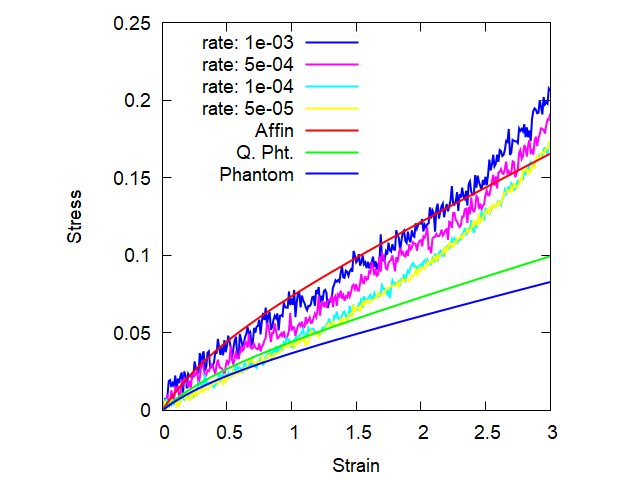
\includegraphics[width=\textwidth]{shear_random_4_N20.png}
%         \caption{Stress-Strain Curves for 4-chain NW at varied shear rate (1e-3 $\sim$ 5e-5 /$\tau$).}
%         \label{fig:deform}
%         \end{center}
%     \end{minipage}
%     \begin{minipage}{0.33\hsize}
%         \begin{center}
%         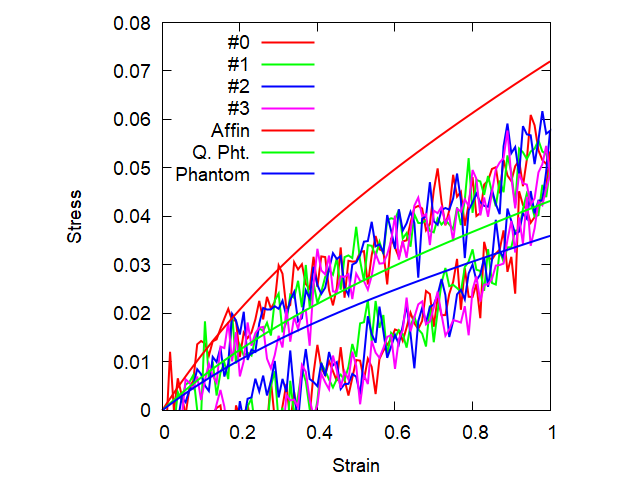
\includegraphics[width=\textwidth]{cyclic_shear_5e-4.png}
%         \caption{Hysteresis Curves for 4-chain NW by Cyclic Shear: shear rate 5e-4}
%         \label{fig:hyst}
%         \end{center}
%     \end{minipage}
%     \begin{minipage}{0.33\hsize}
%         \begin{center}
%         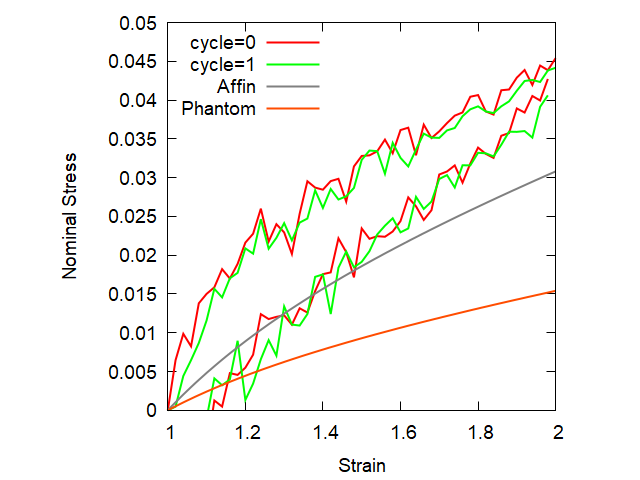
\includegraphics[width=\textwidth]{hyst_4Chain.png}
%         \caption{Strand Exchange Procedure}
%         \label{fig:exc}
%         \end{center}
%     \end{minipage}
% \end{figure}

\begin{figure}[hb]
    \begin{minipage}{0.5\hsize}
        \begin{center}
        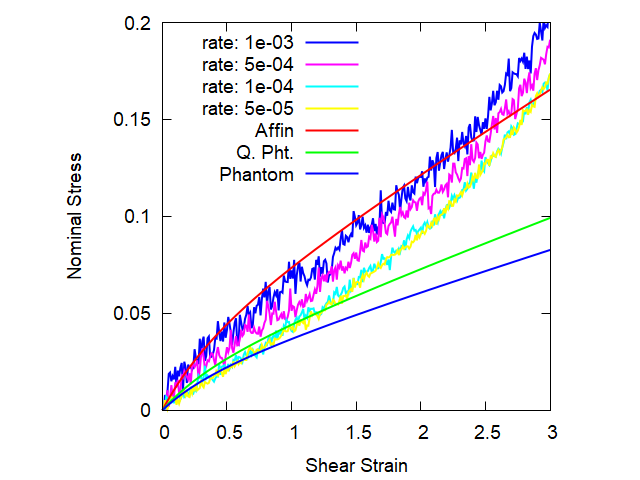
\includegraphics[width=.7\textwidth]{Shear_Random_4chain_N20.png}
        \caption{Stress-Strain Curves for 4-chain NW at varied shear rate (1e-2 $\sim$ 5e-5 $\lambda/\tau$)}
        \label{fig:deform}
        \end{center}
    \end{minipage}
    \begin{minipage}{0.5\hsize}
        \begin{center}
        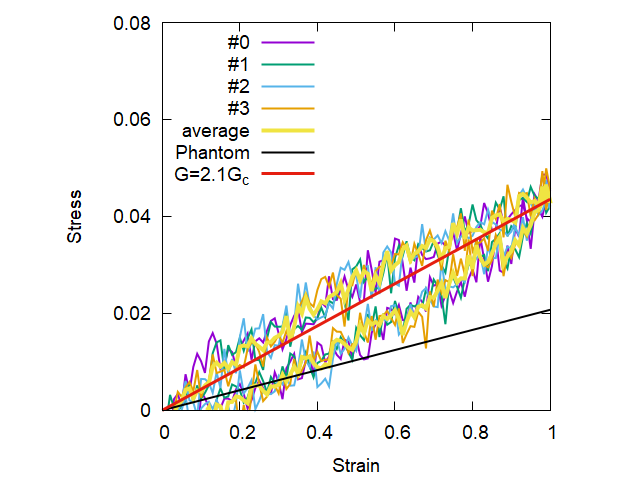
\includegraphics[width=.7\textwidth]{CyclicDeform_4chain_rate_2e-4.png}
        \caption{Hysteresis Curves for 4-chain NW by Cyclic Shear ($\lambda = 1$): shear rate 2e-4 $\lambda/\tau$}
        \label{fig:hyst}
        \end{center}
    \end{minipage}
    % \begin{minipage}{0.33\hsize}
    %     \begin{center}
    %     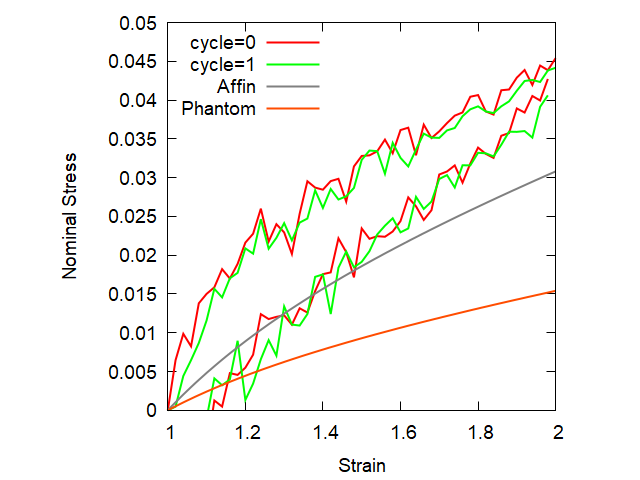
\includegraphics[width=\textwidth]{hyst_4Chain.png}
    %     \caption{Strand Exchange Procedure}
    %     \label{fig:exc}
    %     \end{center}
    % \end{minipage}
\end{figure}

\vspace{-7mm}
\begin{thebibliography}{99}
    \bibitem{andrews} E. H. Andrews, Y. Fukahori Journal of Materials Science, 12, 1307 (1977)
    \bibitem{smith} T. L. Smith, R. A. Dickie Journal of Polymer Science Part A-2: Polymer Physics, 7, 635 (1969)
    \bibitem{flory} P. J. Flory Proceedings of the Royal Society of London. Series A, 351, 351 (1976)
    \bibitem{sasaki} 佐々木裕, 第69回レオロジー討論会 要旨集 (2021)
\end{thebibliography}

\end{document}